\section{LRSCPK for normal estimation}
\label{sec:algorithm}
\subsection{Overview of our algorithm}
{\label{sec:overview}}
With a noisy point cloud $\mathcal{P}=\{p_{i}\}_{i=1}^{N}$ as input, our algorithm takes three steps to estimate the normals, while preserving sharp features. First, we detect the points which are near sharp features. Then, for each of these points, the neighborhood of it is segmented by LRSCPK with prior knowledge estimated from its local structure. Finally, using the segmentation result we select a consistent subneighborhood to estimate the normal. The overall procedure of our method is shown in Fig. \ref{fig:flow_chart}.

%\textbf{Candidate feature points selection.} Normal estimation is challenging in the presence of sharp features. Hence we begin our method with a selection of points which are near sharp features and name them as \emph{candidate feature point}. Using covariance analysis of local neighborhoods, a weight is assigned to each vertex, which measures the likelihood of a vertex belongs to features. Candidate feature point are extracted by eliminating the vertex with low salience weight.
%%We define the threshold automatically. First, we compute
%%a histogram capturing the distribution of the weight $w$. Then the
%%threshold is defined as the horizontal ordinate where the frequency
%%begins to have a slow decrease.
%
%\textbf{Subneighborhood segmentation.} When the point is near sharp features, a neighborhood including distance smooth patches is likely to be got. We perform subspace clustering inside
%the neighborhood of every candidate feature point to identify these patches. All the points in a single cluster represent a smooth region. To robustly segment these intersecting patches, we
%propose a novel subspace clustering method based on structural low
%rank presentation guided by credible regions. Our scheme improve the clustering results by taking both the local information and subspace structure into consideration.
%
%\textbf{Normal estimation} The actual normal estimation applied to a point is
%chosen according to the category of the point.  If a point is not belong to the candidate feature points, the whole neighborhood is used to estimate the normal of the point. Otherwise, we choose the nearest cluster generated by subneighborhood segmentation to estimate the normal.
%As discussed earlier, we would like to identify piecewise
%smooth regions in the neighborhood of each candidate feature point before applying the normal estimation.
%The neighbourhood of each point near sharp features consists multiple smooth surface patches and each patch can be very closely approximated by a plane. Therefore the subspace clustering method proposed in the above section can be used to identify these smooth regions.

\subsection{Candidate feature points selection}
\label{subsec:candidateFeature}
Given a point $p_{i}$, we select a neighborhood $\mathcal {N}_{i}$ of size
$S$ which depends on the noise scale. Then we compute a weight
$w_{i}$ and an
estimated normal $n_{i}$ by covariance analysis of the local
neighborhood. Denote $\lambda_0 \leq \lambda_1 \leq \lambda_2$ as the singular values of the covariance matrix defined in \cite{PaulyKKG03}.
%Let $\hat{p}_{i}$ be the centroid of the local neighborhood, the
%$3\times 3$ covariance matrix $T_{i}$ of $p_{i}$ is defined as
%\begin{equation}\label{eq:pca}
%T=\frac{1}{s}\cdot\left[
%\begin{array}{c}
%p_{i1}-\hat{p}_{i}\\
%\cdots\\
%p_{is}-\hat{p}_{i}\\
%\end{array}
%\right]\cdot\left[
%\begin{array}{c}
%p_{i1}-\hat{p}_{i}\\
%\cdots\\
%p_{is}-\hat{p}_{i}\\
%\end{array}
%\right]^{T},\\
%p_{ij}\in \mathcal {N}_{i},
%\end{equation}
The weight $w_{i}$ is computed as
$$w_{i}=\frac{\lambda_{0}}{\lambda_{0}+\lambda_{1}+\lambda_{2}}.$$
%where the $\lambda_{i}$ are the eigenvalues of $T$ with $\lambda_0 \leq \lambda_1 \leq \lambda_2$.
The normal $n_{i}$ is defined as the eigenvector $v_{0}$ corresponding to the smallest eigenvalue $\lambda_{0}$.

The weight $w_{i}$ measures the confidence of $p_{i}$ belonging to a feature.
If $w_{i}$ is larger than a given threshold $w_{t}$ then $p_{i}$ is regarded as a candidate feature point.
%
Denote the distribution of $\{ w_{i} \}_{i=1}^{N}$ as $f_{w}$ and smooth it by
$$min_{\hat{f}_{w}} \quad \|\hat{f}_{w}-f_{w}\|_{F}+\|Df_{w}\|_{1},$$where $D$ is the second difference matrix, $\|\cdot\|_{F}$ and $\|\cdot\|_{1}$ represent $l_{2}$ norm and $l_{1}$ norm, respectively. We choose the $w_{t}$ after the first peak of the smoothed distribution with gently decrease, as shown in \fig \ref{fig:Candidate_threshold}.
%We choose the $w_{t}$ after the first peak of the $l_{1}$-smoothed distribution of $\{ w_{i} \}_{i=1}^{N}$ with gently decrease, as show in \fig \ref{fig:Candidate_threshold}.
\begin{figure}
  \centering
  % Requires \usepackage{graphicx}
  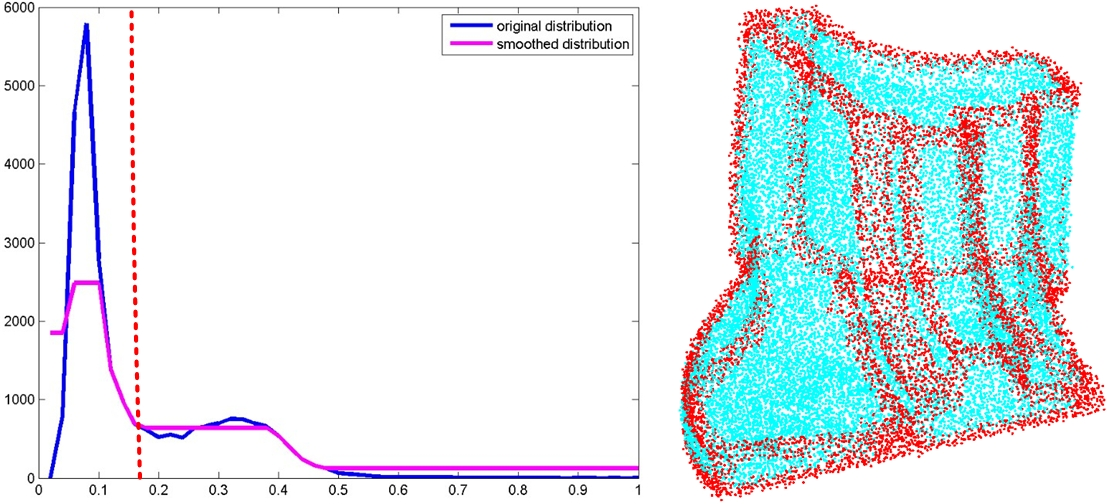
\includegraphics[width=1\linewidth]{feature}
  \caption{The choice of $w_{t}$ (left) and the candidate feature points (right). The red dashed line represent where the threshold is selected }\label{fig:Candidate_threshold}
\end{figure}

\subsection{Subneighborhood segmentation}
\label{sec:Subneighborhood_Segmentation}
\subsubsection{Subneighborhood segmentation by subspace clustering}
For a candidate feature point $p_{i}$, we first select a larger neighborhood $\mathcal {N}_{i}^{*}$ of size $S^{*}$ than $\mathcal{N}_{i}$ used for candidate feature points selection, \ie $S^{*}>S$.
In the local coordinates with $p_{i}$ as the origin, the neighbor point $p_{ij}$ of $p_{i}$ is represented as
$p_{ij} = [x_{j}, y_{j}, z_{j}, n_{xj}, n_{yj}, n_{zj}]',j = 1, \ldots, S^{*},$ where
$[x_{j},y_{j},z_{j}]$ is the coordinate of $p_{ij}\in\mathcal{N}_{i}^{*}$ and
$[n_{xj}, n_{yj}, n_{zj}]$ is its normal computed by PCA.
The sampling matrix is defined as $X = [p_{i1}, p_{i2}, \ldots, p_{iS^{*}}]$.
The optimal coefficient matrix $Z\in \mathbb{R}^{S^{*}\times S^{*}}$ can be computed by solving~\eq~(\ref{eq:RSSLRR}).
After obtaining the affinity matrix from ~\eq~(\ref{eq:defineS}), we segment $\mathcal {N}_{i}^{*}$ by NCut. Since the number of subspaces is unknown, we segment these neighbor points into two classes first.
If any one of them is not a subspace, it is segmented into two classes further.
The iterative progress is terminated until each class is a subspace.

Determining whether or not a class is a subspace is performed by fitting a plane to the class and measuring the average residual.
If the average residual is smaller than a threshold $\tau_{f}$, the class is determined as a subspace.
To automatically compute an appropriate $\tau_{f}$, we compute normalized average residual histograms of candidate feature points and non-candidate points respectively and set $\tau_{f}$ as the horizontal ordinate
where the two histograms cross, as illustrated in \fig \ref{fig:fit_threshold}.
\begin{figure}
  \centering
  % Requires \usepackage{graphicx}
  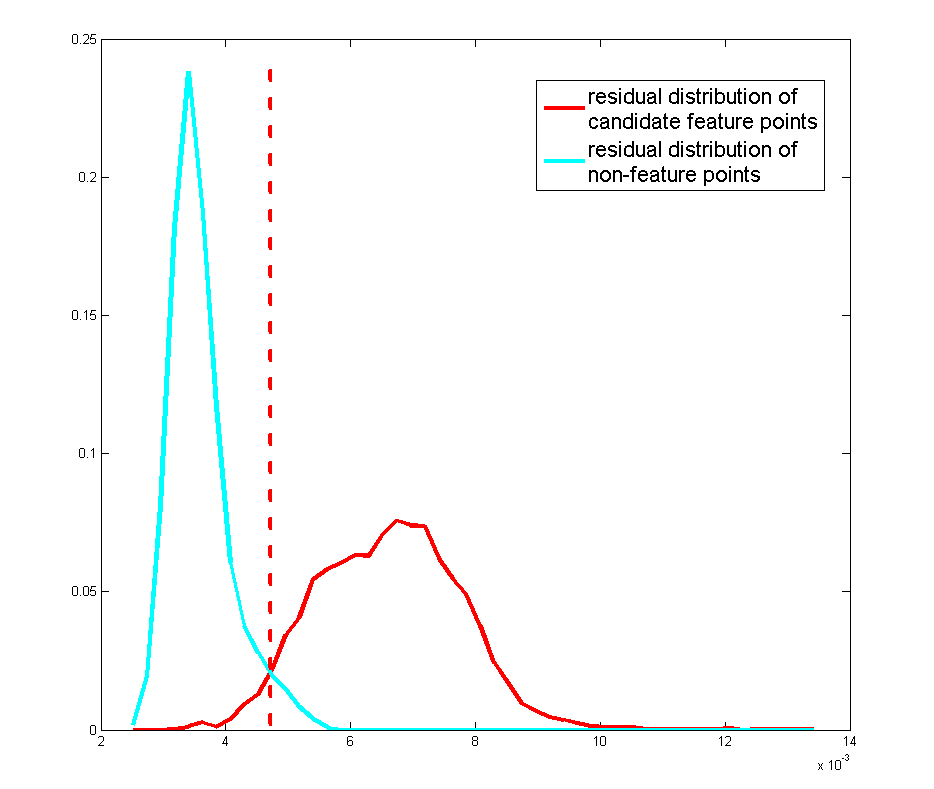
\includegraphics[width=0.9\linewidth]{fit}
  \caption{The choice of $\tau_{f}$. The red dashed line represent where the threshold is selected}\label{fig:fit_threshold}
\end{figure}

\subsubsection{Construction of the guiding matrix}
The guiding matrix $\Omega$ can be built by various ways. We estimate it according to the observation that although normals estimated by PCA are error-prone for points around sharp features, they are reliable for points away from sharp features. Thus the reliable regions are used to guide the segmentation of the neighborhood.
For any two points $p_{ij}$ and $p_{ik}$ in the neighborhood of $p_i$, we compute the normals of $p_{ij}$ and $p_{ik}$ using their $K$-nearest neighbors respectively and compute the distance $D(j,k)$ between the two planes specified by the normals.
If $p_{ij}$ or $p_{ij}$ is adjacent to sharp features, \ie with larger $w_{ij}$ or $w_{ik}$, no plane approximates its neighborhood well. We randomly choose $r$ points from its $K$-nearest neighbors to estimate its normal. The construction of the distance matrix $D$ is shown in \textbf{algorithm} \ref{CDM_pseudocode}.

%Based on the observation that when a point is far from sharp
%features the point and its neighbors often belong to the same
%subspace, we can fit a subspace $\hat{\mathcal {S}}$ by using the
%point and its $K$-nearest neighbors. If two points $j$ and $k$ lie in the same
%subspace $\mathcal {S}_{i}$, their locally estimated subspaces
%$\hat{\mathcal {S}}_{j}$ and $\hat{\mathcal {S}}_{k}$ should be the
%same, while if the two points lie in different subspaces,
%$\hat{\mathcal {S}}_{j}$ and $\hat{\mathcal {S}}_{k}$ should be
%different. Therefore, we can use the distance between $\hat{\mathcal
%{S}}_{j}$ and $\hat{\mathcal {S}}_{k}$ to define a distance matrix
%$D$. However, when the point adjacent to sharp features, the point
%and its neighbors may not belong to the same subspace. Hence, we can
%not directly use the point and its neighbors to fit the subspace.
%Actually there should be some of the neighbors belonging to the same
%subspace with the current point. Therefore we randomly choose $r$
%points from its $K$-nearest neighbors to fit a subspace. The process of constructing
%distance matrix is shown in \textbf{algorithm} \ref{CDM_pseudocode}.
\begin{algorithm}[t]
\linesnumbered \KwIn{\emph{CandidateFeaturePointSet} $A$,
\emph{Non-FeaturePointSet} $B$;} \KwOut{\emph{DistanceMatrix}$D$;}
\BlankLine

\emph{DistanceMatrix} $D=\textbf{0}$;\\
\For{each point $p_{ij} \in A \cup B$} {
    \For{each point $p_{ik} \in A \cup B$}
    {
    \If{$p_{ij} \not\in A $ }
    {
     Normal $n1$ = normal(NearestNeighbors);
     }
    \Else
    {
     Normal $n1$ = normal(RandomNearestNeighbors);
    }
    \If{$p_{ik} \not\in A $ }
    {
     Normal $n2$ = normal(NearestNeighbors);
     }
    \Else
    {
     Normal $n2$ = normal(RandomNearestNeighbors);
    }
    $D(j,k) = 1 - |<n1,n2>|$
    }
}  \caption{Construct The Distance Matrix} \label{CDM_pseudocode}
\end{algorithm}

$D(j,k)$ can be seen as the probability of
points $j$ and $k$ belonging to different planes,~\ie subspaces.
We set $\Omega(j,k) = 1$ if $D(j,k)$ is larger than a threshold $\tau_{max}$, and set $\Omega(j,k) = 0$ otherwise.
%
Denoting $D_{max}$ as the set of the largest $40\%$ elements in the
matrix $D$, we set $\tau_{max} = min(D_{max},1-cos(45^{\circ}))$.
This setting of $\tau_{max}$ means that when the angle between the two estimated planes of $p_{ij}$ and $p_{ik}$ is larger than $45^{\circ}$, they are predicted to belong to different subspaces.

\textbf{Sequence of computing the guiding matrix.}
In order to improve the reliability of the guiding matrix, we first segment neighborhoods of points with smaller $w_i$,
store the segmentation results of each neighborhood and use them to update the guiding matrices of points around sharp features which are computed later.
We denote the number of $p_{ij}$ and $p_{ik}$ in the same
subspace and in different subspaces as $R_{jk}$ and $N_{jk}$, respectively.
If $R_{jk}>N_{jk}$, we define $\Omega(j,k)$ as $\Omega(j,k) = min\left ( \Omega(j,k), 1- \frac{R_{jk}}{R_{jk}+N_{jk}}\times exp(-1/R_{jk}) \right )$.
Otherwise we define $\Omega(j,k)$ as $\Omega(j,k) =
max\left ( \Omega(j,k),\frac{N_{jk}}{R_{jk}+N_{jk}}\times exp(-1/N_{jk}) \right )$.

\textbf{Improvement for points near sharp features.}
When $p_{ij}$ or $p_{ik}$ is near sharp features, the normal estimated using $r$ random points from a point's $K$-nearest neighbors is not reliable.
Therefore the reliability of the probabilities $D(j,:)$ or $D(k,:)$ is lower.
We reduce the corresponding element in the guiding matrix $\Omega$.
Specifically, if only one of $p_{ij}$ or $p_{ik}$ is around sharp features we set $\Omega(j,k) = \alpha \Omega(j,k),$ $0<\alpha<1$.
If both of them are near sharp features we set $\Omega(j,k) = \beta \Omega(j,k),$ $0< \beta < \alpha$.
%
We take $\alpha = 0.6$ and $\beta = 0.2$ in our experiments.
%\begin{algorithm}
%\linesnumbered \KwIn{\emph{CandidateFeaturePointSet} $A$,
%\emph{Non-FeaturePointSet} $B$,\emph{DistanceMatrix} $D$;}
%\KwOut{\emph{GuidingMatrix}$\Omega$;} \BlankLine
%
%\emph{GuidingMatrix} $\Omega=\textbf{0}$;\\
%\For{each point $p_i \in A \cup B$} {
%    \For{each point $p_j \in A \cup B$}
%    {
%    \If{$D(i,j) > threshold$ }
%    {
%      \If{$p_i \not\in A$ and $p_j \not\in A$}
%      {
%      $L(i,j) = 1$
%      }
%      \If{$p_i \in A$ and $p_j \in A$}
%      {
%      $L(i,j) = \alpha$
%      }
%      \If{($p_i \not\in A$ and $p_j \in A$) or ($p_i \in A$ and $p_j \not\in A)$}
%      {
%      $L(i,j) = \beta$
%      }
%    }
%    }
%}  \caption{Construct The Leading Matrix} \label{CLM_pseudocode}
%\end{algorithm}

\subsection{Normal estimation}
For the non-candidate points, their neighborhood is isotropic and normals estimated by PCA is used. For any candidate feature point $p_i$, its neighborhood is anisotropic. We segment its neighborhood into several isotropic subneighborhoods by the method described in section \ref{sec:Subneighborhood_Segmentation}.
For each subneighborhood, a plane is fitted to $p_i$ and the subneighborhood.
Thus each subneighborhood has a fitting residual. The subneighborhood with the minimum residual is identified as a consistent subneighborhood of $p_i$. Then an accurate normal can be easily estimated using the consistent subneighborhood.

%Denoting $n$ as the number of points and $n_{f}$ as the number of candidate feature points, the complexity of our method, RNE and HF are $O(n\mathrm{log}n + n_{f}\times s^{*3})$, $O(n\mathrm{log}n)$ and $O(n\mathrm{log}n)$, respectively.
\subsection{Time complexity of our algorithm}
\label{sec:timing}
Our algorithm takes three steps: candidate feature points selection, subneighborhood segmentation and normal estimation. The time complexity of them are $O(N\mathrm{log}N)$, $O(N_{f}\times(\mathrm{log}N + (S^{*})^{3}))$ and $O(N_{f}\mathrm{log}N)$, respectively, where $N$ is the number of points and $N_{f}$ is the number of the candidate feature points.
%-
We use Kd-tree for neighborhood search (the $\mathrm{log}N$ factor) and repeat some local operations for each point (the N factor) in the first step and for each candidate feature point (the $N_{f}$ factor) in the remaining steps.
%-
For each candidate feature point, the most time-consuming operation is to solve ~\eq~(\ref{eq:RSSLRR}) when segmenting  subneighborhood of size $S^{*}$. A modified alternating direction method (ADM) is designed with the same complexity of the standard one \cite{convergence} (the $(S^{*})^{3}$ factor) and presented in Appendix 1.
%
Thus the time complexity of our algorithm is $O(N\mathrm{log}N + N_{f}\times (S^{*})^{3})$.
%{\color{blue}The complexity of solving ~\eq~(\ref{eq:RSSLRR}) can be reduced to $O((S^{*})^{2})$ using the linearized alternating direction approach \cite{LinLS11}.} \jz{The parallel computing can be employed further to speed up our algorithm.(could delete)}
